\subsubsection{Epena-Gruppe}\label{sec:EPE-Gr}

Die Epena-Gruppe\footnote{Die entsprechende Keramik wurde bis Ende 2015 als \enquote{Jeke}-Gruppe systematisiert und auch in der Veröffentlichung \textcite[119 Fig. 6-3, 123]{Seidensticker.2016b} so bezeichnet. Erst Ende 2015 wurde durch die Lektüre der Arbeit von \textcite[27--36]{MpikaNgoma.1996} die Herstellung von entsprechenden Gefäßen in Epena (Fpl.~306) nachgewiesen. Diese war vorher lediglich durch Hinweise im Feldbuch Eggert (06.\,05.\,1987 sowie 11.\,05.\,1987) anzunehmen.} beschreibt die rezenten keramischen Formen, die 1987 bei der Prospektion des \mbox{Likwala}-\mbox{aux}-\mbox{Herbes} beobachtet wurden. Die der Epena-Gruppe zugerechneten GE stammen nur zu kleinen Teilen aus ausgegrabenen Kontexten.\footnote{Vier GE wurden bei der Grabung eines rezenten Grabes (Kat.-Nr.~14) in Boleko am unteren \mbox{Likwala}-\mbox{aux}-\mbox{Herbes} (Fpl.~285) erfasst und eine weitere GE stammt aus der ebenfalls rezenten Grube PIK~87/2 (Kat.-Nr.~9) in Pikunda am mittleren \mbox{Sangha} (Fpl.~255).} Das Gros der GE (99\,\%) stammt aus Surveys, die in den Dörfern durchgeführt wurden. Insgesamt wurden 354~GE aufgenommen (60\,\%). Aufgrund der Fragmentierung und wiederkehrenden Merkmals-Kombination wurden 240 weitere Scherben typologisch angesprochen und ausgezählt (40,\%).\footnote{Die ausgezählten Stücke umfassen fast ausschließlich Randscherben (139 Stücke) sowie Wandungsfragmente (92 Stücke) und stammen ausschließlich von Fundstellen entlang des Likwala-aux-Herbes, dem Hauptverbreitungsgebiet der Epena-Keramik.} Insgesamt konnten 251 GE sicher der Epena-Gruppe zugewiesen werden (72\,\%), während bei 99 weiteren GE aufgrund ihrer starken Fragmentierung eine Zuweisung nur unter Vorbehalt möglich war (28\,\%). Das aufgenommene Material der Epena-Gruppe umfasst 24 komplette oder hinreichend komplette Gefäße, die jedoch nur etwa 4\,\% des gesamten Inventars ausmachen. Die meisten dieser Gefäße stammen aus Mosenge (Fpl.~299; 7 GE) und Itanga (Fpl.~305; 7 GE). Das Gros der GE der Epena-Gruppe bilden Randfragmente (56\,\%). Teile von Gefäßwandungen machen lediglich 36\,\% aus und 4\,\% konnten als Bodenstücke angesprochen werden. Die Herstellung von Gefäßen der Epena-Gruppe in Epena am oberen \mbox{Likwala}-\mbox{aux}-\mbox{Herbes} (Fpl.~306) ist durch Léopold \textsc{Mpika-Ngoma} (1996: 27--36) belegt.\footnote{Die Herstellung des Halses einer Flasche vom Typ A4 wird in mehreren, leider schlecht reproduzierten Fotografien wiedergegeben (\textsc{Mpika-Ngoma} ebd. 28--31). Überdies wird ein Ensemble aus sechs Gefäßen (ebd. 32 oben) sowie das Umwickeln einer großen Flasche (Typ A3) mit einem Geflecht aus Palmblätten (ebd. 32 unten) illustriert. Über den Nutzen dieses zuletzt genannten Schrittes werden keine Ausführen gemacht. Siehe Anm.~\ref{ftn:EthnoToepfereiInVorb}.} Im 3\,km von Epena entfernt gelegenen Dorf Mabongo wurde ebenfalls rezente Keramik der Epena-Gruppe dokumentiert (ebd. 35).\footnote{Es handelt sich um eine Flasche des Typs A3 sowie ein weitmundiges, hohes Gefäß vom Typ B2 (\textsc{Mpika-Ngoma} 1996: 35).}

\paragraph{Technologische Merkmale}\hspace{-.5em}|\hspace{.5em}%
Die Keramik der Epena-Gruppe ist in der technischen Tradition des Inneren Kongobeckens hergestellt. Insgesamt 95\,\% aller GE sind den \textit{Fabrics} 1 oder 2 zuzurechnen, da sie keine (81\,\%) bis kaum (15\,\%) nichtplastische Partikel aufweisen. Konnten Partikel beobachtet werden, handelte es sich fast ausschließlich um Quarzpartikel der Größenklassen \textit{very fine} (72\,\%) oder \textit{fine} (17\,\%). Die Färbung der GE deutet auf eine vornehmliche Nutzung weißbrennender Tone (67\,\%) hin, während Hinweise für die Verwendung rotbrennender Tone sehr selten zu beobachten waren (8\,\%). Diese sehr deutliche Homogenität der GE der Epena-Gruppe mit Blick auf die untersuchten technologischen Eigenschaften spiegelt sich auch in den Anteilen einzelner \textit{Fabrics} wider. Es dominieren die Varianten 1d (36\,\%) sowie 1b (32\,\%), während die \textit{Fabrics} 1c und 1a (je 10\,\%) bereits deutlich seltener vorkommen.

\begin{figure*}[!tb]
	\centering
	\includegraphics[width=\textwidth]{fig/EPE-Typen.pdf}
	\caption{Epena-Gruppe: Typvertreter.\\1:~Taf.~95.1; 2:~Taf.~80.9; 3:~Taf.~88.3; 4:~Taf.~86.1; 5:~Taf.~96.1; 6:~Taf.~86.2; 7:~Taf.~85.4; 8:~Taf.~79.7; 9:~Taf.~79.9; 10:~Taf.~85.8; 11:~Taf.~85.7; 12:~Taf.~78.4.}
	\label{fig:EPE_Typentafel}
\end{figure*}

\paragraph{Formen}\hspace{-.5em}|\hspace{.5em}%
Das Spektrum an Gefäßformen innerhalb der Epena-Gruppe wird von drei grundlegenden Typen bestimmt: hohe Gefäße mit kurzem Kegelhals und schmalem Schulterabsatz (Typ~B4; 26\,\%; Taf.~79.6--7,79.9--10,80.1,81.3--4,81.6--8,81.10--11,85.4,86.4)\footnote{Die GE unterscheiden sich von jenen der Ebambe-Gruppe eigentlich nur durch die Abwesenheit von \textit{banfwa-nfwa}-Verzierungen.}, Flaschen mit profilierter Wandung und breitem Schulterabsatz (A3; 24\,\%; Abb.~\ref{fig:EPE_Typentafel}.3,6, Taf.~69.3, 69.5 82.10, 84.7--8, 85.1, 88.2, 97.4) sowie schalenförmige Gefäße mit abknickender Wandung und zylindrischem Oberteil (G4; 16\,\%; Taf.~78.4--7). Daneben finden sich in den Inventaren hohe Gefäße mit weiten Halsbereichen und stark profilierten Gefäßwandungen (Typ~B2--3; 17\,\%; Abb.~\ref{fig:EPE_Typentafel}.1--2,4--5) sowie schalenförmige Gefäße mit einem Absatz unterhalb des Randes (Typ~G2; 6\,\%; Abb.~\ref{fig:EPE_Typentafel}.11). Ebenfalls vertreten sind flache Gefäße mit geschweifter Wandung und einem Absatz unterm Rand (Typ~E6; 6\,\%) sowie schalenfömrige Gefäße mit abknickender Wandung, einem geraden Unter- und konkavem Oberteil (Typ~G3; 3\,\%). Bei zwei Drittel aller GE war die Gefäßform sicher anzusprechen.

\begin{figure*}
	\begin{minipage}[b]{\columnwidth}
		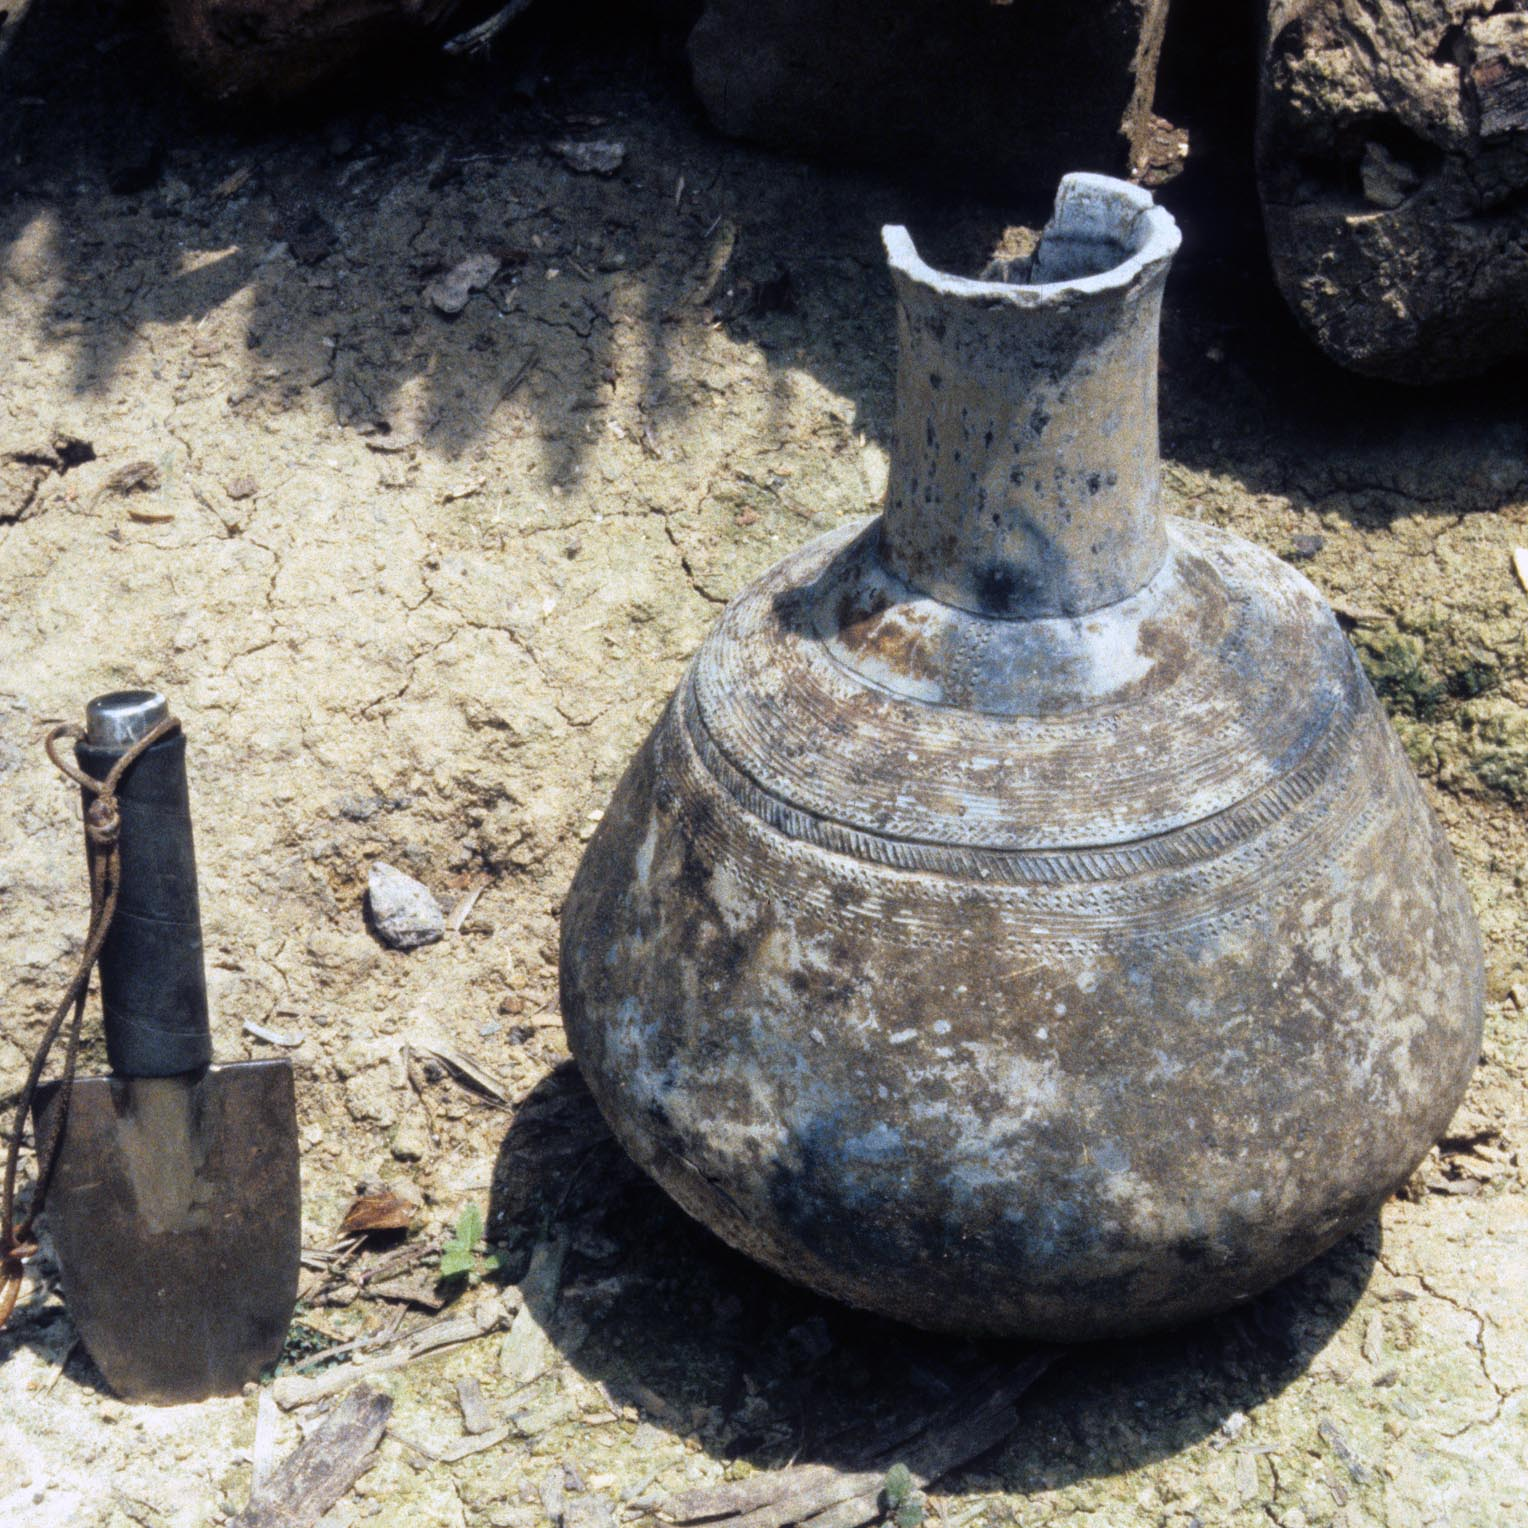
\includegraphics[width=\textwidth]{fig/MUN87-101_E87-036-3.jpg}
	\end{minipage}\hfill
	\begin{minipage}[b]{\columnwidth}
		\caption{Munda (Fpl.~304): Flasche vom Typ A3 (Foto: M.~K.~H. Eggert, 1987).}\label{fig:MUN87-101_EPE-Flasche}
	\end{minipage}
\end{figure*}

Mit Blick auf die Proportionen der Epena-Gefäße sind zwei Gruppen zu unterscheiden: die schalenförmigen Gefäße sind regelhaft etwa doppelt so breit (10--42\,cm) wie hoch (5,5--10\,cm). Da knapp 48\,\% der Schalen der Epena-Gruppe lediglich im Randbereich ließ sich die Mündungshöhe jedoch nur selten rekonstruieren. Bei fast allen hohen Gefäßen mit Schulterabsatz und Kegelhals (B4) ließ sich die Höhe der Mündung nicht ermitteln. Die wenigen GE, die eine Rekonstruktion zuließen, deuten ein Verhältnis zwischen maximalem Durchmesser und Mündungshöhe von 1:1,5 an. Die flaschenförmigen Gefäße vom Typ A3 weisen regelhaft einen großen Bauchdurchmesser auf, der zwischen 10--34\,cm liegt, bei einer Höhe von 11--41\,cm. Die Höhe dieser Gefäße ist häufig nur 20--25\,\% größer als ihr maximaler Durchmesser.

\begin{figure*}[p]
	\centering
	\includegraphics[width=\textwidth]{fig/EPE_Verbreitung.pdf}
	\caption{Epena-Gruppe: Verbreitung.}
	\label{fig:EPE_Verbreitung}
\end{figure*}

Die Ränder der Epena-Gefäße sind entweder ausbiegend (B1; 29\,\%) oder zylindrisch (A1; 28\,\%). Eine sehr spezifische Variante der ausbiegenden Ränder weist einen konvexen Verlauf auf (15\,\%; Taf. 85.4--5, 94.6, 95.4). Es handelt sich hierbei um eine Variante der einfach ausbiegenden, leicht verdickten Ränder des Typs B1, die innerhalb des eng mit der Epema-Gruppe verwandten Ebambe-Stils (Kap.~\ref{sec:EBA-Gr}) regelhaft zu beobachten sind. Kurze sowie lange Varianten ausbiegender Ränder (B1.1--B1.2) konnten bei 6--10\,\% der Randstücke beobachtet werden. Die Randlippen sind zu einem überwiegenden Teil gerade abgestrichen (M3; 66\,\%). Schräg nach innen oder außen abgestrichene Randlippen wurden nur bei jeweils 9--10\,\% der Randstücke beobachtet. Abgerundete sowie spitze Randlippen (M1--2) kommen deutlich seltener, nur bei 4--8\,\% der Randstücke vor.

Bei 31 GE war eine Identifikation des Gefäßbodens möglich. Das Gros dieser GE weist flache Böden auf (74\,\%), wobei die einfachen, flachen Standböden vom Typ B4 mit 65\,\% den Großteil ausmachen. Runde Böden finden sich nur sehr selten im Fundgut der Epena-Gruppe (19\,\%) und ließen sich lediglich bei den sehr selten vorkommenden, flachen Gefäßen mit geschweifter Wandung vom Typ E1 sowie den charakteristischen schalenförmigen Gefäßen mit abknickender Wandung und zylindrischem Oberteil vom Typ G4 beobachten. Alle übrigen Gefäßformen sind regelhaft mit flachen Böden assoziiert (Abb.~\ref{fig:EPE_Typentafel}.1,4--6,10). Böden mit konkaver Standfläche (B6) konnten nur selten beobachtet werden (3\,\%; Abb.~\ref{fig:EPE_Typentafel}.11).

\paragraph{Verzierungen}\hspace{-.5em}|\hspace{.5em}%
Die GE der Epena-Gruppe weisen nur selten Verzierungen auf. Insgesamt 31\,\% aller der Epena-Gruppe zugeordneten GE zeigen kein Dekor und über 75\,\% aller Stücke weisen zwei oder weniger Verzierungselemente auf. Die bestimmenden Verzierungselemente sind Riefen und Rillen, die zusammen 78\,\% ausmachen. Allein horizontale Rillen (Tab.~\ref{tab:Verzierungselemente}: 02.1) machen 47\,\% aller Verzierungselemente aus. Zickzack-Linien (Tab.~\ref{tab:Verzierungselemente}: 01.6; 9\,\%) sowie \textit{Schachbrett}-Muster aus diagonalen Ritzlinien (Tab.~\ref{tab:Verzierungselemente}: 01.2; 8\,\%) stellen innerhalb der Riefen- und Rillen-Verzierungen die häufigsten Verzierungselemente nach den horizontalen Rillen dar. Durch Eindrücke erzielte Verzierungen machen etwa 20\,\% aller Verzierungselemente aus. Eine häufige Variante sind horizontale Reihen aus diagonal gestellten Eindrücken (Tab.~\ref{tab:Verzierungselemente}: 04.12; 10\,\%). Verzierungen beschränken sich auf die Hals- sowie Schulterbereiche der Gefäße (Anlage~4\subref{fig:EPE_Verz}). Insgesamt finden sich etwa 82\,\% aller aufgenommenen Verzierungselemente in diesen beiden Gefäßzonen. Die Standflächen sind regelhaft unverziert.

\paragraph{Datierung}\hspace{-.5em}|\hspace{.5em}%
Für die Epena-Keramik liegen keine absoluten Datierungen vor. Die Keramik wurde bei der Befahrung des Likwala-aus-Herbes 1987 in Benutzung angetroffen, wobei Gefäße fotografisch dokumentiert wurden (Abb.~\ref*{fig:MUN87-101_EPE-Flasche}). Noch in den 1990er Jahren wurde die Herstellung von Gefäßen der Epena-Gruppe in Epena durch \textsc{Mpika-Ngoma} (ebd. 27--36) dokumentiert. Die Epena-Gruppe beschreibt das rezente Spektrum der 1987 genutzten und produzierten Keramik entlang des Likwala-aux-Herbes.

\paragraph{Verbreitung}\hspace{-.5em}|\hspace{.5em}%
Das Verbreitungsgebiet der Epena-Keramik lässt sich im Kern durch den 1987 prospektierten, etwa 500\,km langen Abschnitt des \mbox{Likwala}-\mbox{aux}-\mbox{Herbes} beschreiben (Abb.~\ref*{fig:EPE_Verbreitung}). Entlang der gesamten Strecke fanden sich bei Surveys moderner Dorfflächen GE der Epena-Gruppe. Darüber hinaus fand sich lediglich in Leme (Fpl.~269) am Oberlauf des \mbox{Sangha} ein hohes Gefäß mit weitem und langem Halsbereich sowie stark profilierter Gefäßwandung vom Typ~B2 (Taf.~61.16). Vereinzelt ließ sich Keramik der Epena-Gruppe auch an Fundorten im Mündungsbereich des \mbox{Sangha}, genauer in Bonga (Fpl.~238) sowie Bobusa (Fpl.~239) und in Sungu (Fpl.~236) und Gombe (Fpl.~237) am Kongo nachweisen. Entlang des \mbox{Likwala}-\mbox{aux}-\mbox{Herbes} wurde von der lokalen Bevölkerung angegeben, dass entsprechende Keramik lediglich in Epena am Oberlauf des Flusses (Fpl.~306) produziert würde. Es handelt sich bei der Epena-Keramik mutmaßlich um ein den \mbox{Likwala}-\mbox{aux}-\mbox{Herbes} stromab verhandeltes Produkt der am eponymen Fundort seinerzeit noch betriebenen Töpferei.\footnote{Entsprechende Angaben machte die lokale Bevölkerung in Sosolo (Fpl.~241) am 06.\,05.\,1987 sowie in Ifondo (Fpl.~253) am 11.\,05.\,1987 (Feldbuch M.~K.~H. Eggert 1987).}